\documentclass[parskip=full]{scrartcl}

\pdfoutput=1

\usepackage{breakcites}
\usepackage[square,numbers]{natbib}
\usepackage{float}
\usepackage{graphicx}
\usepackage{geometry}
\geometry{%
	a4paper,
	left=18mm,
	right=18mm,
	top=18mm,
}
\usepackage{amsmath}
\usepackage{enumitem}
\usepackage[ruled,vlined]{algorithm2e}
\usepackage{booktabs}
\usepackage{pgfplotstable}
\pgfplotsset{compat=1.14}
\usepackage{longtable}
\usepackage{tabu}
\usepackage{hyperref}
\date{}

\definecolor{hypecol}{HTML}{0875b7}
\hypersetup{%
    colorlinks,
    linkcolor={hypecol},
    citecolor={hypecol},
    urlcolor={hypecol}
}

\title{%
    Active Learning Augmentation
}

\author{%
	Joao Fonseca\(^{1*}\), Fernando Bacao\(^{1}\)
	\\
	\small{\(^{1}\)NOVA Information Management School, Universidade Nova de Lisboa}
	\\
	\small{*Corresponding Author}
	\\
	\\
	\small{Postal Address: NOVA Information Management School, Campus de
    Campolide, 1070--312 Lisboa, Portugal}
	\\
	\small{Telephone: +351 21 382 8610}
}

\begin{document}

\maketitle

\begin{abstract}
    Abstract goes here.
\end{abstract}

\section{Introduction}

Introduction goes here.

\section{Active Learning Methods}

Review on Data Augmentation Methods go here.

\section{Data Augmentation Methods}

Review on Data Augmentation Methods go here.

\section{Proposed Method}

\section{Methodology}~\label{sec:methodology}

This section describes the different elements included in the experimental
procedure. The datasets used were acquired in open data repositories and its
sources and preprocessing steps are defined in Subsection~\ref{sec:datasets}.
The choice of classifiers used in the experiment are defined in
Subsection~\ref{sec:machine_learning_algorithms}. The metrics chosen to
measure AL performance and overall classification performance are defined in
Subsection~\ref{sec:evaluation_metrics}. The experimental procedure is
described in Subsection~\ref{sec:experimental_procedure}. The implementation
of the experiment and resources used to do so are described in
Subsection~\ref{sec:software_implementation}.

The methodology developed serves purposes: (1) Compare classification
performance once all the AL procedures are completed (\textit{i.e.,} optimal
performance of a classifier trained via iterative data selection) and (2)
Compare the amount of data required to reach specific performance thresholds
(\textit{i.e.,} number of AL iterations required to reach similar the optimal
classification performance).

\subsection{Datasets}~\label{sec:datasets}

The datasets used to test the proposed method are publicly available in open
data repositories. Specifically, they were retrieved from
\href{https://www.openml.org/}{OpenML} and the
\href{https://archive.ics.uci.edu/}{UCI Machine Learning Repository}. The
datasets were chosen considering different domains of application, all of them
focused on classification tasks. The goal is to demonstrate the performance of
the different AL frameworks in various scenarios and domains. The data
preprocessing approach was similar across all datasets.
Table~\ref{tab:datasets_description} describes the key properties of the 10
preprocessed datasets where the experimental procedure was applied. 

\begin{table}[H]
    \centering
    \addtolength{\leftskip} {-2cm}
    \addtolength{\rightskip}{-2cm}
    \pgfplotstabletypeset[
        col sep=comma,
        string type,
        every head row/.style={%
            before row=\toprule,
            after row=\midrule
        },
        every last row/.style={after row=\bottomrule},
    ]{../analysis/datasets_description.csv}
    \caption{\label{tab:datasets_description}
        Description of the datasets collected from each corresponding scene.
        The sampling strategy is similar to all scenes.
    }
\end{table}

The data preprocessing procedure is depicted as a flowchart in
Figure~\ref{fig:data_preprocessing}.

\begin{figure}[H]
	\centering
	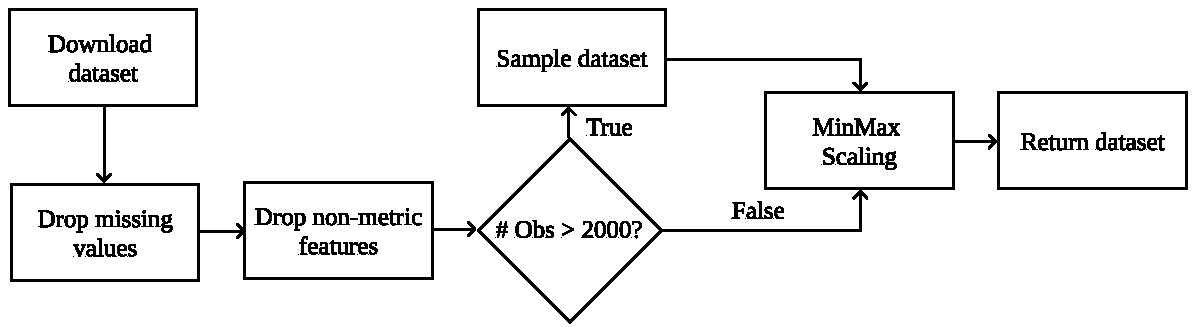
\includegraphics[width=1\linewidth]{../analysis/data_preprocessing}
    \caption{%
        Data preprocessing pipeline.
    }~\label{fig:data_preprocessing}
\end{figure}

\subsection{Machine Learning Algorithms}~\label{sec:machine_learning_algorithms}

Classifiers and generators used.

\subsection{Evaluation Metrics}~\label{sec:evaluation_metrics}

Performance metrics.

\subsection{Experimental Procedure}~\label{sec:experimental_procedure}

Experimental procedure.

\subsection{Software Implementation}~\label{sec:software_implementation}

The experiment was implemented using the Python programming language, along
with the Python libraries
\href{https://scikit-learn.org/stable/}{Scikit-Learn}~\cite{Pedregosa2011},
\href{https://imbalanced-learn.org/en/stable/}{Imbalanced-Learn}~\cite{JMLR:v18:16-365},
\href{https://geometric-smote.readthedocs.io/en/latest/?badge=latest}{Geometric-SMOTE}~\cite{Douzas2019},
\href{https://cluster-over-sampling.readthedocs.io/en/latest/?badge=latest}{Cluster-Over-Sampling}~\cite{Douzas2018},
\href{https://research-learn.readthedocs.io/en/latest/?badge=latest}{Research - Learn}
and
\href{https://mlresearch.readthedocs.io/en/latest/?badge=latest}{ML-Research}
libraries. All functions, algorithms, experiments and results are provided in
the \href{https://github.com/joaopfonseca/ml-research/}{GitHub repository of
the project}.

\section{Results \& Discussion}~\label{sec:results_discussion}

\subsection{Results}~\label{sec:sub_results}


% TODO: Captions need to be rewritten

\begin{table}[H]
    \centering
    \pgfplotstabletypeset[
        col sep=comma,
        string type,
        every head row/.style={%
            before row=\toprule,
            after row=\midrule
        },
        every last row/.style={after row=\bottomrule},
    ]{../analysis/mean_std_aulc_ranks.csv}
    \caption{%
        Mean rankings of the AULC metric over the different datasets (7),
        folds (5) and runs (3) used in the experiment. This means that the use
        of G-SMOTE almost always improves the results of the original
        framework.
    }\label{tab:aulc_ranks}
\end{table}


\begin{table}[htb]
    \centering
    \pgfplotstabletypeset[
        col sep=comma,
        string type,
        every head row/.style={%
            before row=\toprule,
            after row=\midrule
        },
        every last row/.style={after row=\bottomrule},
    ]{../analysis/mean_std_aulc_scores.csv}
    \caption{\label{tab:aulc_scores}
        Average AULC of each AL configuration tested. Each AULC score is
        calculated using the G-mean scores of each iteration in the validation
        set. By the end of the iterative process, each AL configuration used a
        total of 750 instances of the 960 instances that compose the training
        set.
    }
\end{table}

\begin{table}[H]
    \centering
    \addtolength{\leftskip} {-2cm}
    \addtolength{\rightskip}{-2cm}
    \pgfplotstabletypeset[
        col sep=comma,
        string type,
        every head row/.style={%
            before row=\toprule,
            after row=\midrule
        },
        every last row/.style={after row=\bottomrule},
    ]{../analysis/optimal_data_utilization.csv}
    \caption{\label{tab:optimal_data_utilization}
        Mean data utilization of AL algorithms, as a percentage of the
        training set.
    }
\end{table}

\begin{figure}[H]
	\centering
	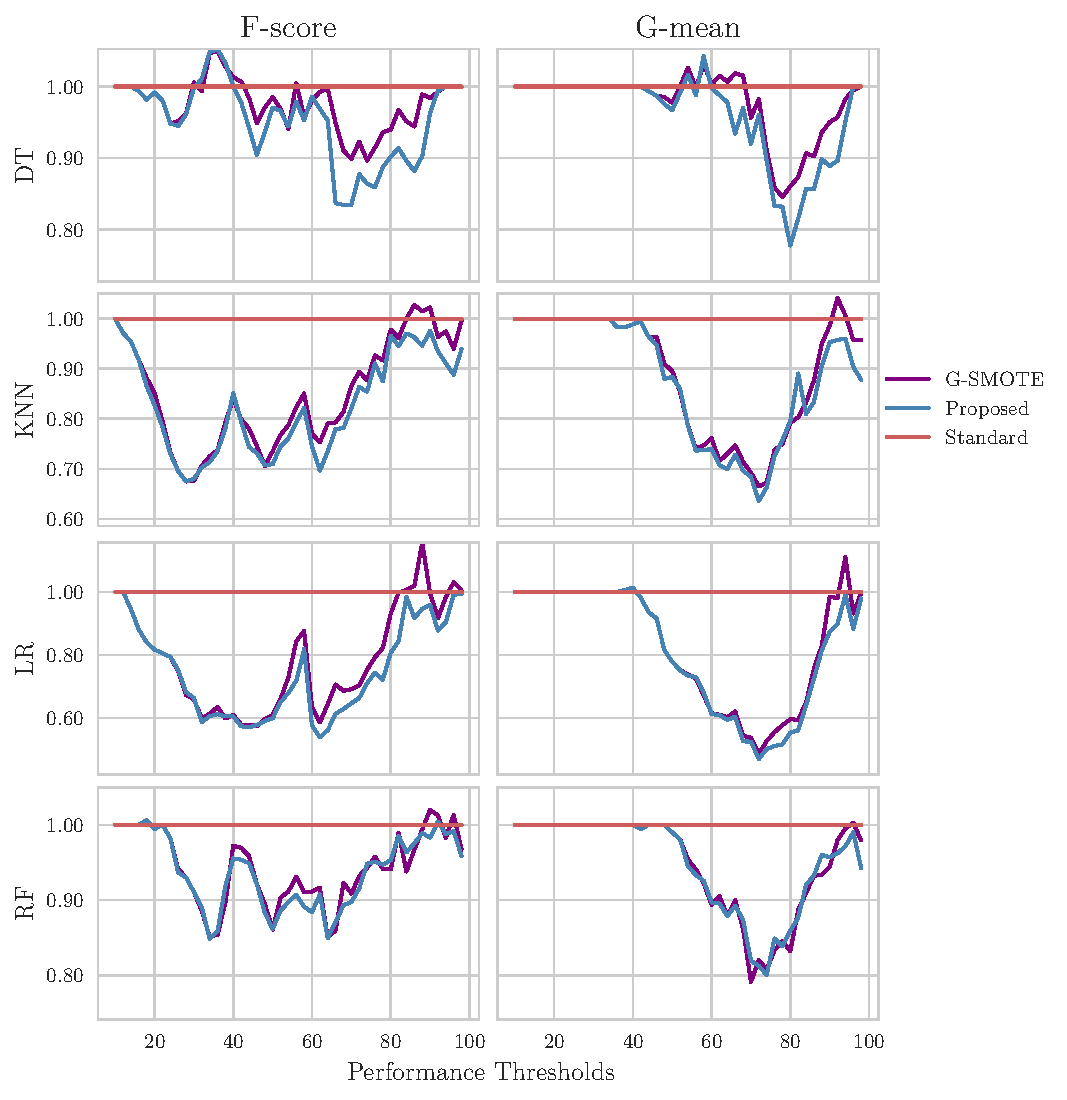
\includegraphics[width=1\linewidth]{../analysis/data_utilization_rate}
    \caption{%
        Mean data utilization rates. The y-axis shows the percentage of data
        (relative to the baseline AL framework) required to reach the
        different performance thresholds.
    }~\label{fig:dur}
\end{figure}


\begin{table}[H]
    \centering
    \addtolength{\leftskip} {-2cm}
    \addtolength{\rightskip}{-2cm}
    \pgfplotstabletypeset[
        col sep=comma,
        string type,
        every head row/.style={%
            before row=\toprule,
            after row=\midrule
        },
        every last row/.style={after row=\bottomrule},
    ]{../analysis/optimal_mean_std_scores.csv}
    \caption{\label{tab:optimal_mean_std_scores}
        Optimal classification scores. The Maximum Performance (MP)
        classification scores are calculated using classifiers trained using
        the entire training set.
    }
\end{table}


% \begin{table}[H]
%     \centering
%     \pgfplotstabletypeset[
%         col sep=comma,
%         string type,
%         every head row/.style={%
%             before row=\toprule,
%             after row=\midrule
%         },
%         every last row/.style={after row=\bottomrule},
%     ]{../analysis/wide_optimal_aulc.csv}
%     \caption{\label{tab:wide_optimal_aulc}
%         AULC scores of each AL configuration tested over the different
%         datasets. Each AULC score is calculated using the G-mean scores of
%         each iteration in the validation set. By the end of the iterative
%         process, each AL configuration used a total of 750 instances of the
%         960 instances that compose the training set.
%     }
% \end{table}


\subsection{Statistical Analysis}~\label{sec:statistical-analysis}


\begin{table}[htb]
	\centering
    \pgfplotstabletypeset[
        col sep=comma,
        string type,
        every head row/.style={%
            before row=\toprule,
            after row=\midrule
        },
        every last row/.style={after row=\bottomrule},
    ]{../analysis/wilcoxon_test.csv}
    \caption{%
    	Adjusted p-values using the Wilcoxon signed-rank method. Bold values
        are statistically significant at a level of $\alpha = 0.05$. The 
        null hypothesis is that the performance of the proposed
        framework is similar to that of the original framework.
    }\label{tab:wilcoxon_test}
\end{table}

% TODO: add analysis of dataset complexity versus AL performance


\subsection{Discussion}~\label{sec:sub_discussion}

\section{Conclusion}~\label{sec:conclusion}


\bibliography{references}
\bibliographystyle{ieeetr}

\end{document}
